\section{Simulations}\label{sec:simulations}

There are two main randomized simulation scenarios inside simulation module 
(module described in \ref{subsec:simulations-architecture}).
First simulation is designed to be static.
It creates only one execution plan
and then it shut downs.
The second simulation reflects the presumed production environment
and is described in the figure \ref{fig:simulation-process}.

\begin{figure}[ht] 
	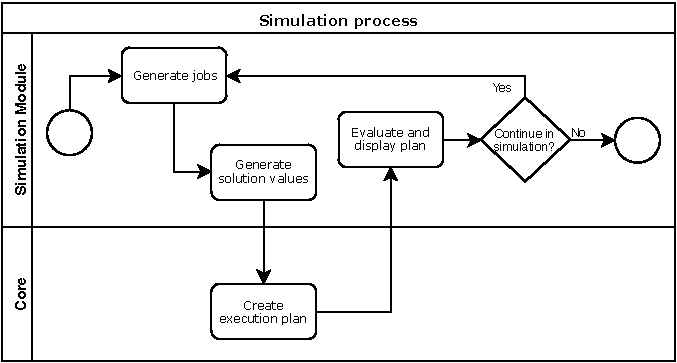
\includegraphics[width=\textwidth]{i_simulation_process.pdf} 
	\centering
	\caption{Simulation process}
	\label{fig:simulation-process}
\end{figure}

Simulation's output (produced execution plan) is printed to standard output.
Data displayed in listing~\ref{lst:data-example} are an exact output produced by the simulation with 5 jobs being scheduled at once.
The optimization jobs,
which were scheduled in the listing~\ref{lst:data-example},
have their parameters displayed in the table~\ref{table:jobs-parameters}

\begin{table}[h]
	\centering
	\caption{Table with jobs parameters}
	\begin{tabular}{|c|c c c c c|} 
		\hline
		Job ID   & 0      & 1     & 2     & 3     & 4     \\
		\hline\hline
		$D^{j}$  & 284    & 161   & 373   & 271   & 129   \\
		\hline
		$P^{j}$  & 757    & 42    & 73    & 51    & 29    \\
		\hline\hline
		Duration & 180    & 120   & 360   & 240   & 120   \\
		\hline
    Cost     & 131.20 & 24.36 & 65.08 & 39.16 & 28.48 \\
    \hline
	\end{tabular}
	\label{table:jobs-parameters}
\end{table}
 
\begin{lstlisting}[caption={Simulation data output},label={lst:data-example},language=Kotlin]
    0 iteration:
                Times:||  0| 60|120|180|240|300|360|
    ----------------- || --|---|---|---|---|---|---|
        Cost: 1 + 0.02||  2|  2|  4|  3|  3|  2|  2|
        Cost: 1 + 0.02||  2|  2|  4|  3|  3|  2|  2|
        Cost: 1 + 0.02||  2|  2|  4|  3|  3|  2|  2|
        Cost: 1 + 0.02||  3|  4|  4|  3|  3|  2|  2|
        Cost: 1 + 0.02||  4|  4|  4|  3|  3|  2|  2|

      Cost: 1.5 + 0.02||  1|  1|  1|  2|   |   |   |
      Cost: 1.5 + 0.02||  1|  1|  1|  2|   |   |   |

     Cost: 10.0 + 0.05||  0|  0|  0|  0|   |   |   |
     Cost: 10.0 + 0.05||  0|  0|  0|  0|   |   |   |

    Total plan cost: CostImpl(value=264.587)$
\end{lstlisting}

\bigskip \noindent
\inlinecode{Times} axis shows time units ($t$ value described in section \ref{sec:formal-definition}) in seconds.
Second, vertical axis, visualizes resources.
Name, \inlinecode{Cost: 1 + 0.02} is name of the resources provider (explained in section \ref{subsec:formalized-definition-representation}),
and each line is one usage unit - meaning that it could be one physical core or for example percentage of shared processor.
In implementation, this value is referred as CPU core,
but in fact, it is dimensionless value expressing usage of some system resources.

Each cell contains either number or is empty.
Number is job ID and indicates, that this resource is allocated to job with displayed ID.
This is effectively $^{r}x_{t}^{j}$ value explained in section \ref{subsec:variables-definition}.

Total plan cost is sum of all particular costs of all jobs - their resources allocations.
Therefore this is the cost of created plan.